\documentclass{beamer}

\usepackage{hyperref}
\usepackage{verbatim}
\usepackage{textpos}
\usepackage{multicol}


\title{DIME Beamer Template}
\author{Add your name here}
\institute{DIME - World Bank}
\date{\today}

\begin{document}
\begin{frame}
	
\includegraphics[width=\textwidth]{img/Header.png}
	\vspace{-0.2cm}
	\titlepage 	 
\end{frame}
%\frame{\titlepage \vspace{-0.2cm}

%\frame{
%	\frametitle{Overview}
%	\tableofcontents
%}

\addtobeamertemplate{frametitle}{}{%
\begin{textblock*}{\linewidth}(0cm,8cm)
		
\includegraphics[width=\linewidth]{img/Footer.png}
\end{textblock*}}

\begin{frame}{Add items}	

\begin{itemize}
	\item Currently, a lot of us, export tables from Stata and then copy paste the tables on to Excel and then to Word or something similar. 
	\item {\LaTeX} allows us to create a document once and every time a do-file is run, the tables are automatically updated in our {\LaTeX} document.
	\item This saves us a lot of time in the long run even though the learning curve for {\LaTeX} is a bit complicated compared to MS Word. 
	
\end{itemize}
\end{frame}

\begin{frame}{Add items sequentially}	

	\begin{itemize}
		\item<1->Currently, a lot of us, export tables from Stata and then copy paste the tables on to Excel and then to Word or something similar. 
		\item<2->{\LaTeX} allows us to create a document once and every time a do-file is run, the tables are automatically updated in our {\LaTeX} document.
		\item<3->This saves us a lot of time in the long run even though the learning curve for {\LaTeX} is a bit complicated compared to MS Word. 
		
	\end{itemize}
\end{frame}


\begin{frame}{Add image}	

	\begin{figure}
		\centering
		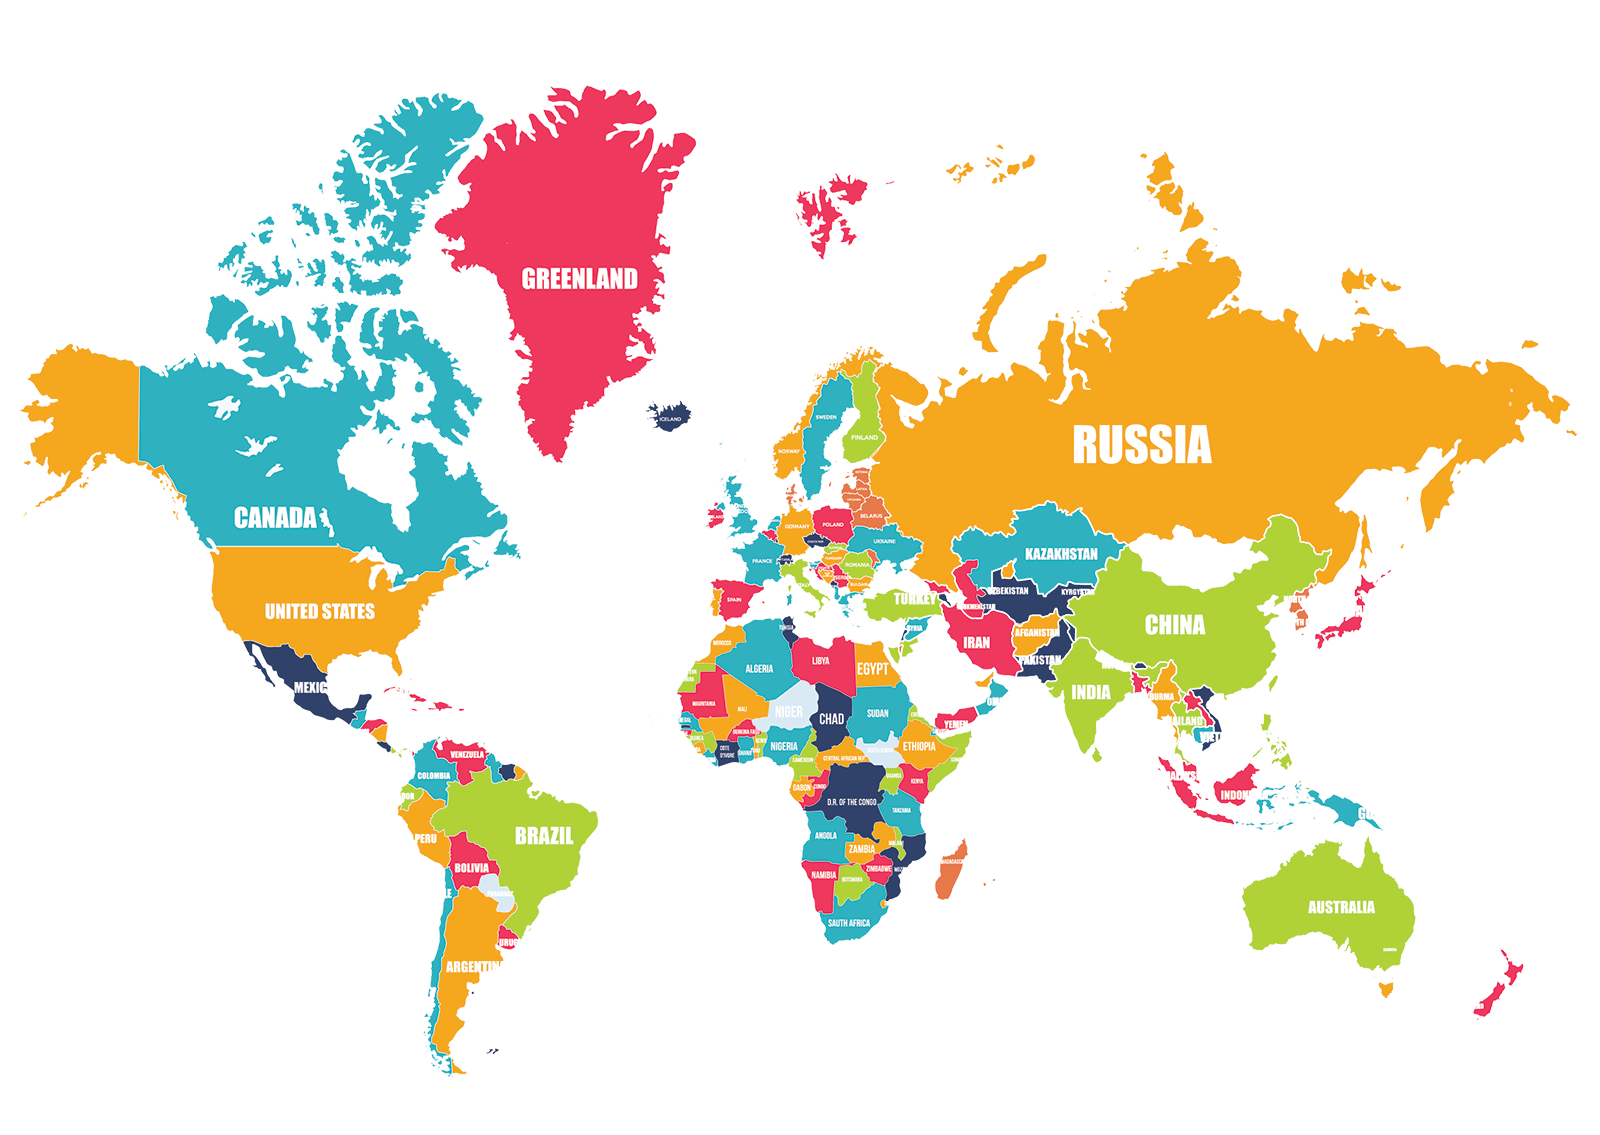
\includegraphics[width=.8\linewidth]{img/world-map}
		\caption{World map}
		\label{fig:world-map}
	\end{figure}
	
\end{frame}

\begin{frame}{Add more than one image}

You can also display two images side by side

	\begin{multicols}{2}
		
		\begin{figure}
			\centering
			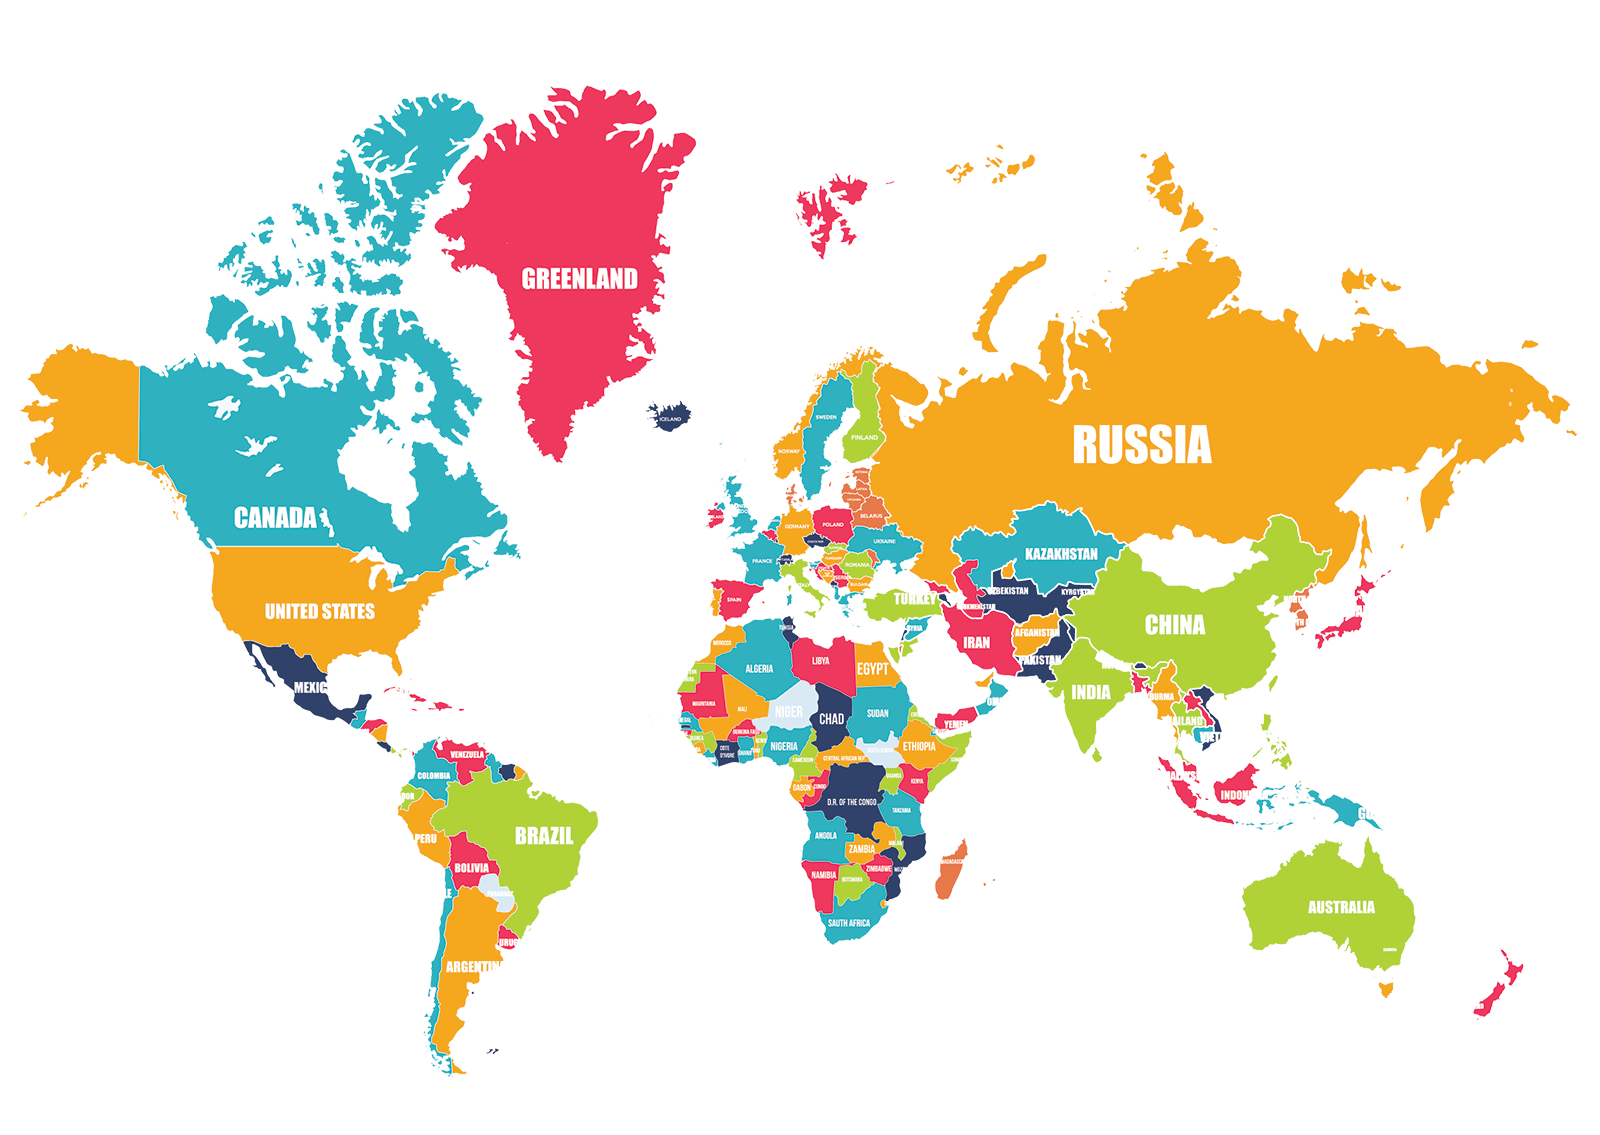
\includegraphics[width=\linewidth]{img/world-map}
			\caption{World map 1}
			\label{fig:world-map1}
		\end{figure}
		\begin{figure}
			\centering
			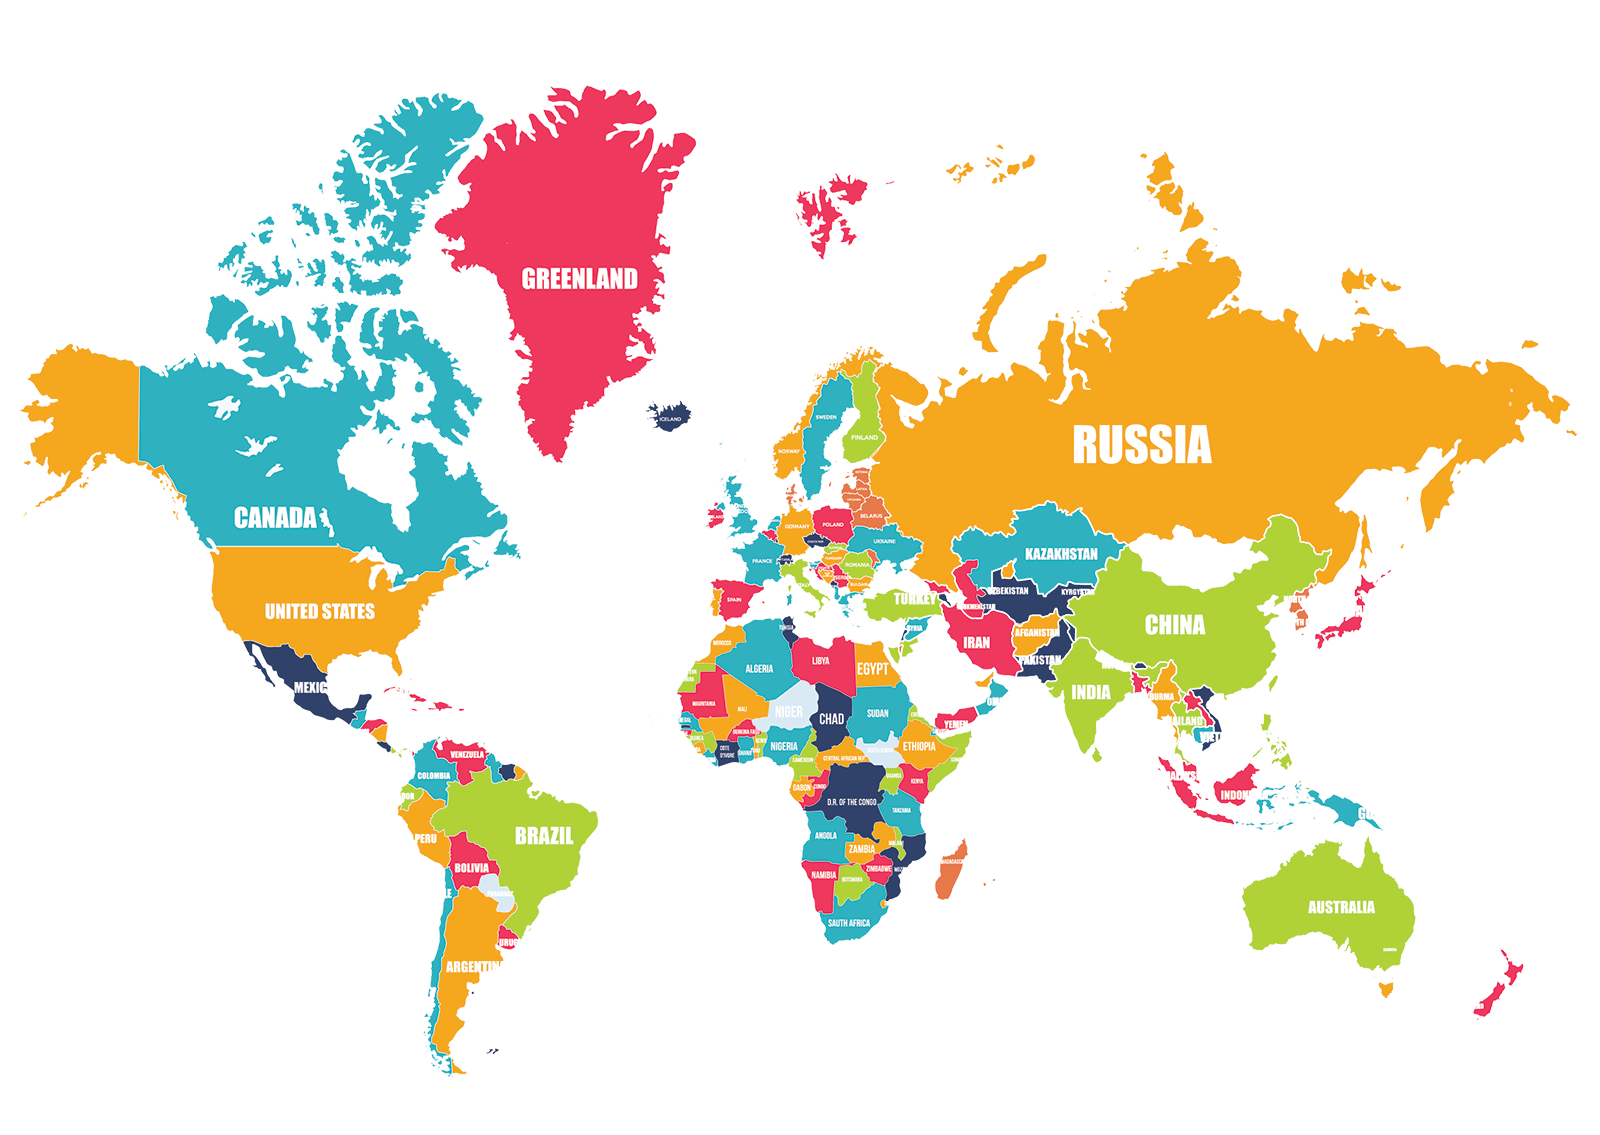
\includegraphics[width=\linewidth]{img/world-map}
			\caption{World map 2}
			\label{fig:world-map2}
		\end{figure}
	
	\end{multicols}

\end{frame}

\begin{frame}{Add image and text}

Lorem ipsum dolor sit amet, consectetur adipiscing elit

	\begin{multicols}{2}
		
		\begin{itemize}
			\item Mauris ut justo aliquam, consequat diam vitae, hendrerit felis
			\item Suspendisse ullamcorper tincidunt posuere
			\item Quisque vitae ipsum in massa commodo mattis
		\end{itemize}
		\begin{figure}
			\centering
			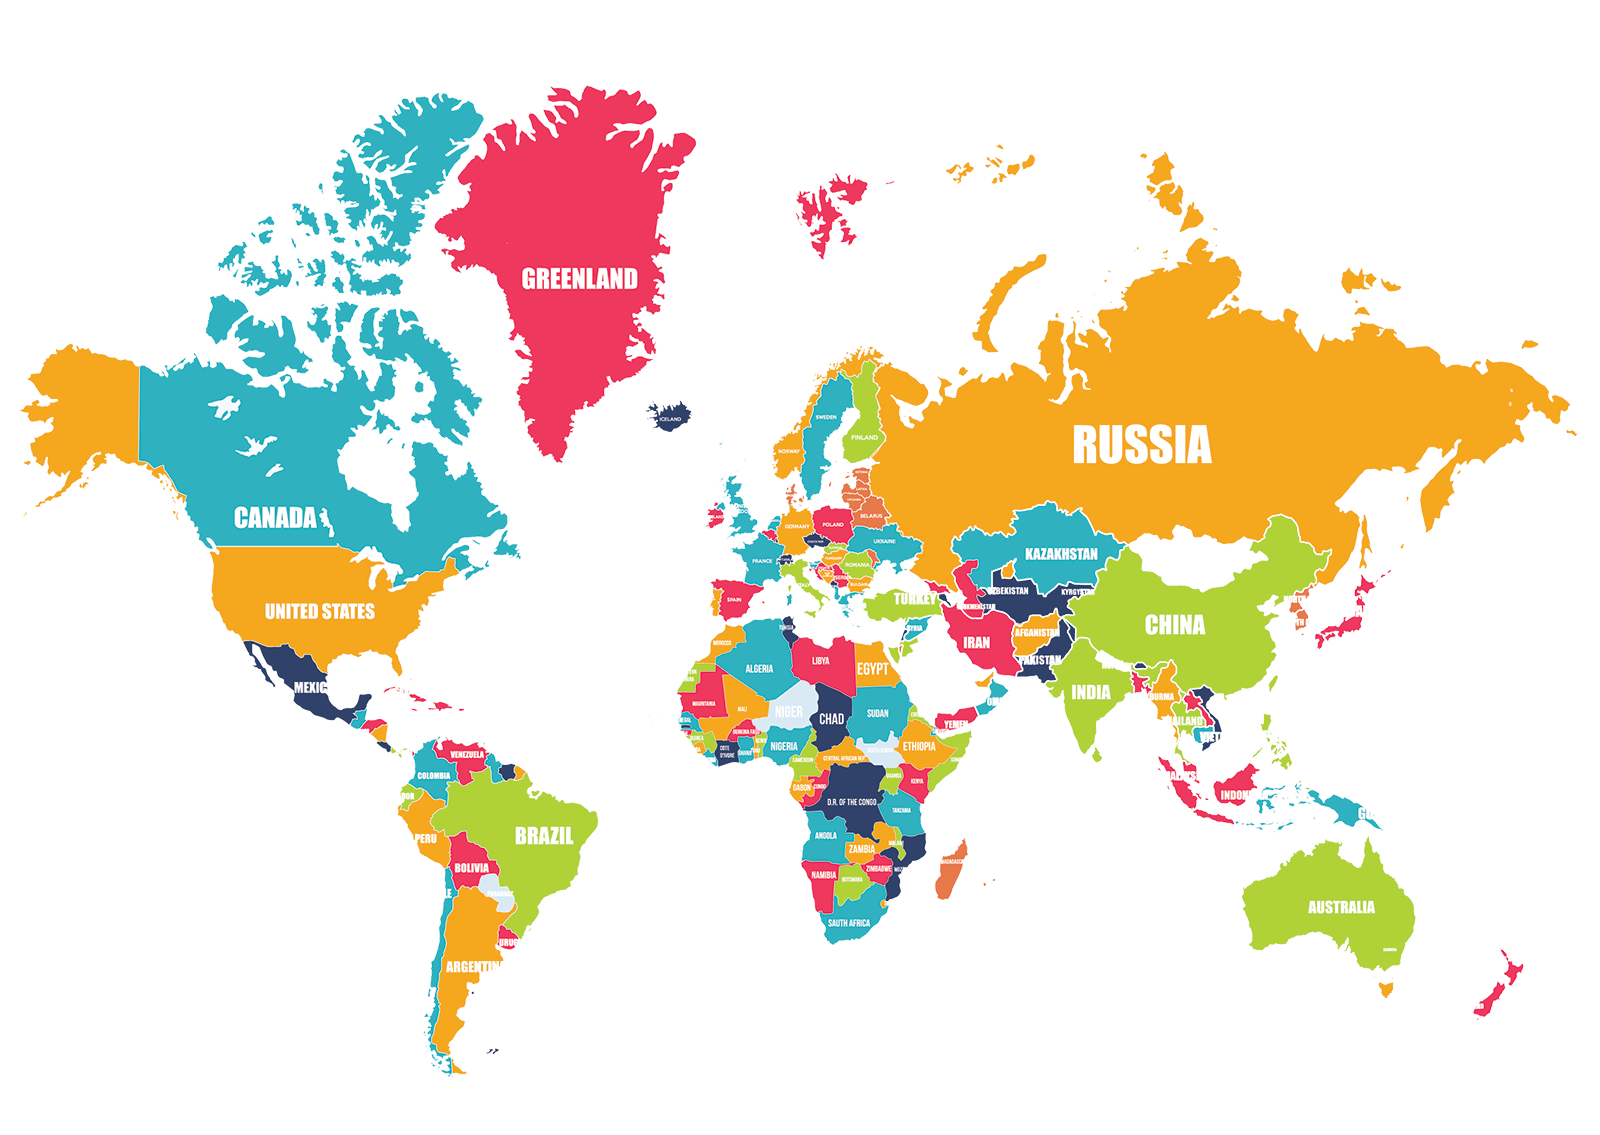
\includegraphics[width=\linewidth]{img/world-map}
			\caption{World map 3}
			\label{fig:world-map3}
		\end{figure}
		
	\end{multicols}

\end{frame}

\begin{frame}
	\centering\Huge\textcolor{orange}{\textbf{Thank you!}}
\end{frame}

\begin{frame}{References}
	\begin{tiny}\bibliography{bibliography}\end{tiny}
\end{frame}


\end{document}
